%% Author: Giacomo Minello

% The document class
% \documentclass{report}
% \documentclass{book}
\documentclass[12pt]{article}
 
\usepackage{graphicx}
\graphicspath{ {./figures/} }
% babel english 
\usepackage[english]{babel}
%allow H on figures
\usepackage{float}

\usepackage{csquotes}

%indent chapters
\usepackage{indentfirst}


\setlength{\headheight}{14.5pt}

%allow subfigures
\usepackage{subcaption}

\usepackage{fancyhdr}
\pagestyle{fancy}
%references done right
\usepackage[
backend=biber,
sorting=none
]{biblatex}
\addbibresource{references/biblio.bib}

% cross-referenced element become links 
\usepackage[hidelinks]{hyperref}

%This will set the options to configure the behaviour of the links within the document. 
%Every parameter must be comma-separated and the syntax must be in the format parameter=value. 
\hypersetup{
    colorlinks=false,
    %linkcolor=black,
    %urlcolor=cyan,
    %pdftitle={PDF title},
    %pdfpagemode=FullScreen
}
\urlstyle{same}

\setlength{\parskip}{0.5em}
 

\title{The Stuxnet attack on the Natanz fuel enrichment plant in Iraq\\
\large{Post attack analysis in a cyberwarfare scenario}
\rule[0.1cm]{13cm}{0.1mm}
\rule[0.5cm]{13.5cm}{0.6mm}}
\author{Group: Nuclear Pizza Toppings \\
Nicolò Diomedi, Gabriele Gallotti, Giacomo Minello
\\
\scriptsize‘‘[…] whoever provided the required intelligence may as well know the favorite pizza toppings \\
\scriptsize of the local head of engineering.’’\cite{killcentrifuge}
\\
}

% Set today date
\date{\today}
%set date to null to avoid showing it in maketitle
\date{}

\begin{document}
\begin{titlepage}
% create title
\maketitle
\begin{abstract}
\noindent  This document aims to provide an holistic view of the Stuxnet cyber attack on the Natanz fuel enrichment plant.

\noindent In the first part of this document we will provide a description of the plant and of the context in which it functioned.

\noindent We will then illustrate the actual attack, the way in which it worked, and we will try to explain why it was so successful in its endeavour.
\end{abstract}
\end{titlepage}


% table of content 
\tableofcontents

\listoffigures

\newpage

\section{Introduction}
Natanz ({نطنز}) is a hardened Fuel Enrichment Plant (FEP) covering 100,000 square meters that is built 8 meters underground and protected by a concrete wall 2.5 meters thick, itself protected by another concrete wall. In 2004, the roof was hardened with reinforced concrete and covered with 22 meters of earth. The complex consists of two 25000 square meter halls and a number of administrative buildings. This once secret site was one of the two exposed by Alireza Jafarzadeh in August, 2002. IAEA Director General Mohamed ElBaradei visited the site on 21 February 2003 and reported that 160 centrifuges were complete and ready for operation, with 1000 more under construction at the site. Under the terms of Iran’s safeguards agreement, Iran was under no obligation to report the existence of the site while it was still under construction.

\begin{figure*}[ht!]
    \centering
    \begin{subfigure}[t]{0.5\textwidth}
        \centering
        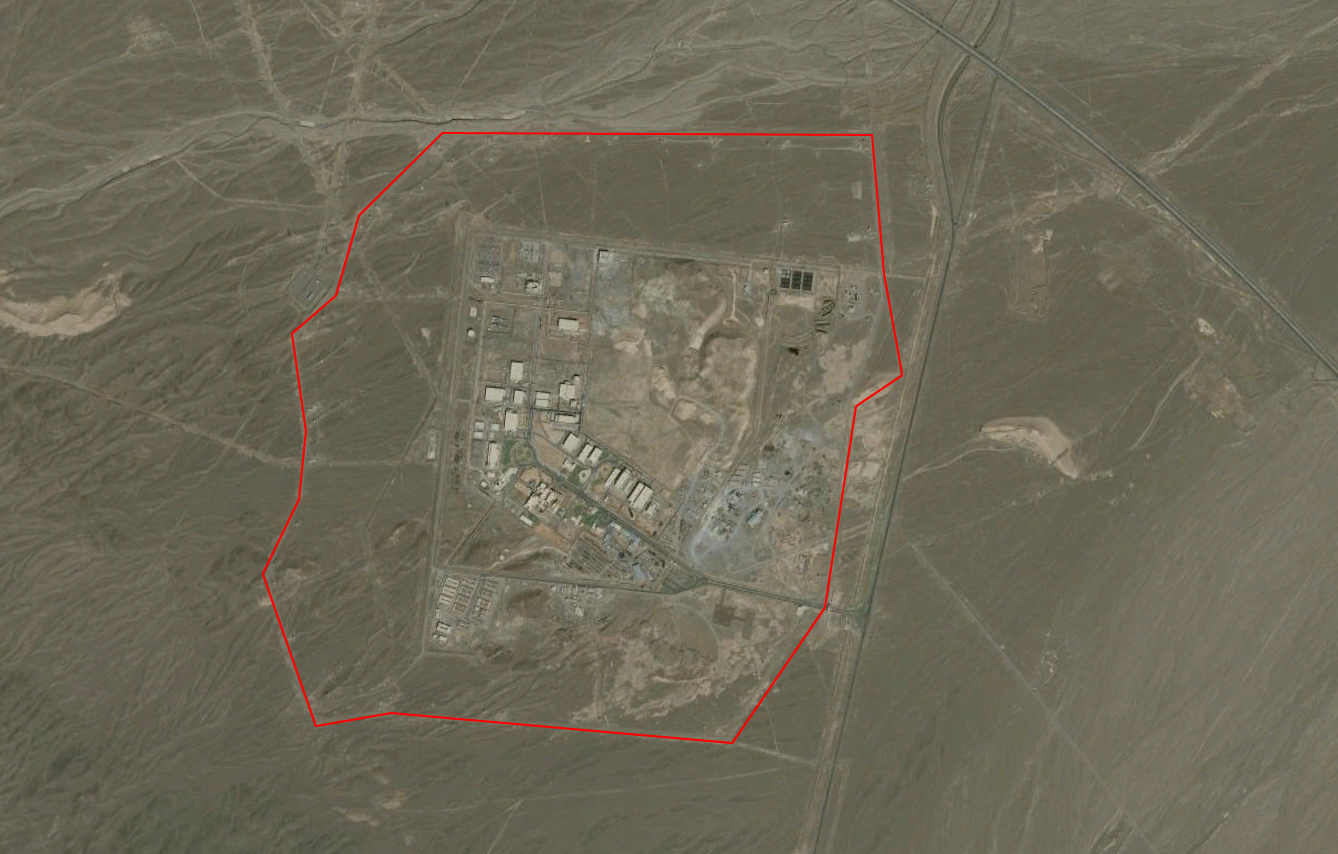
\includegraphics[height=0.65\textwidth]{natanz1.jpg}
        \caption{Highlighted: 4.7 miles security perimeter}
    \end{subfigure}%
    ~ 
    \begin{subfigure}[t]{0.5\textwidth}
        \centering
        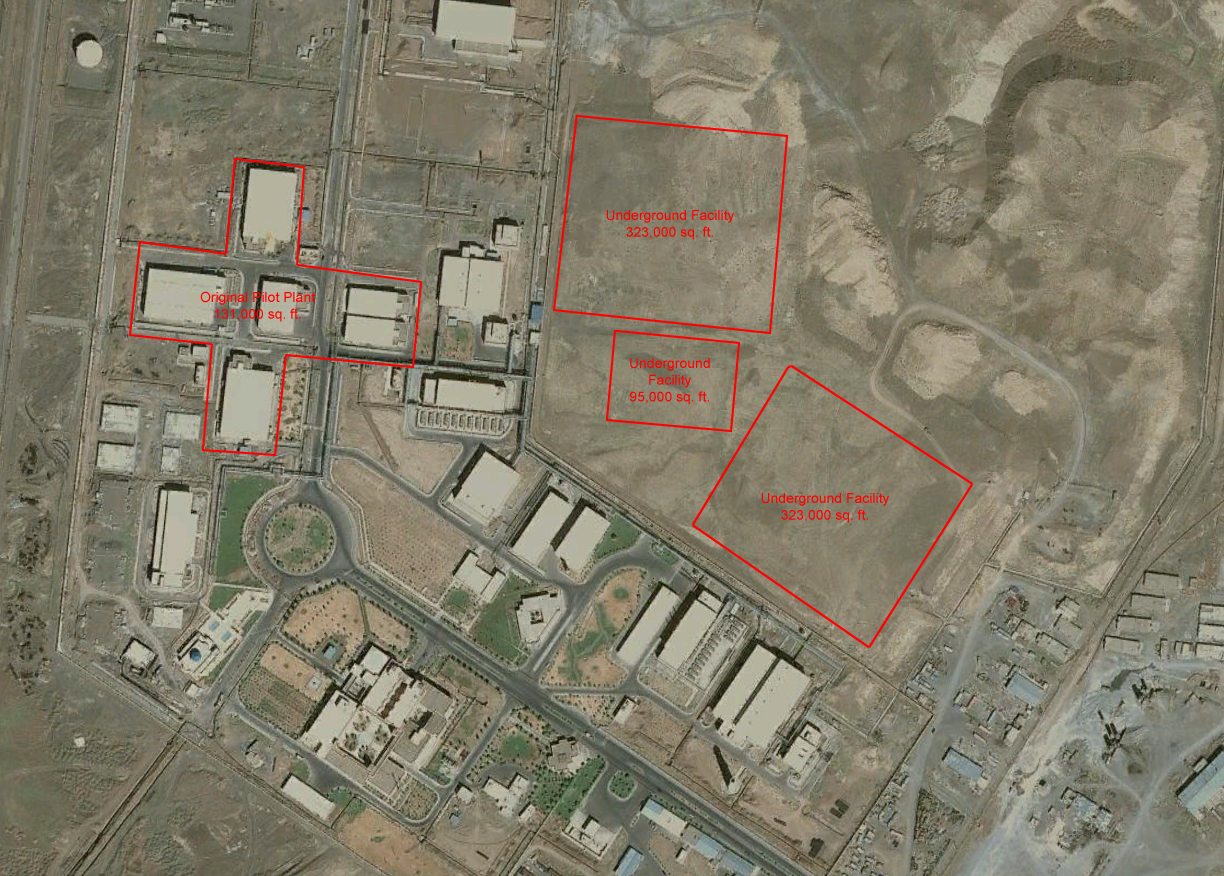
\includegraphics[height=0.65\textwidth]{natanz2.jpg}
        \caption{Buildings complex and underground structures}
    \end{subfigure}
    \caption{Natanz Fuel Enrichment Plant satellite images. \href{https://publicintelligence.net/iran-nuclear-site-natanz-uranium-enrichment-site/}{Source.}}
\end{figure*}

    TO DO: add Geopolitical context.

\section{Description of the system}
    \begin{figure}[H]
    \centering
    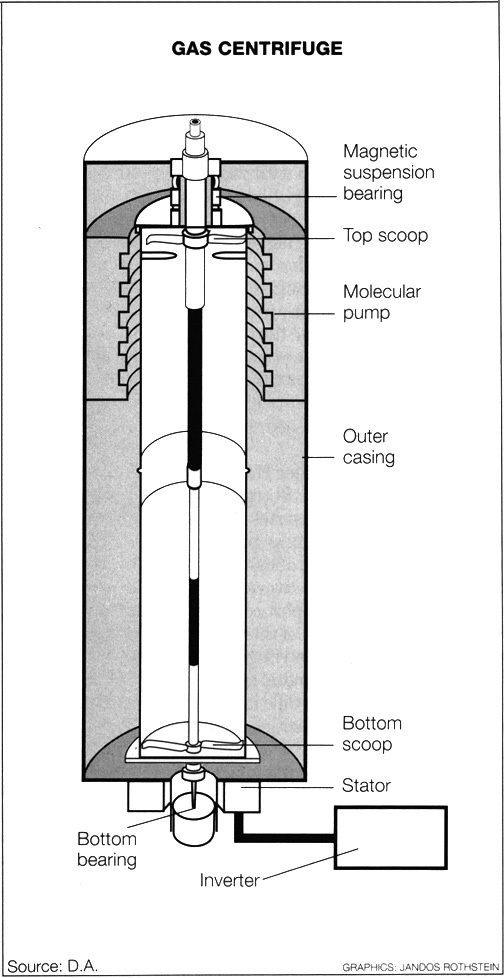
\includegraphics[height=0.65\textwidth]{figures/centrifugeAlternative.jpg}
    \caption{Centrifuge}
    \label{fig:centrifuge1}
    \end{figure}
The backbone of Iran’s uranium enrichment effort is the IR-1 centrifuge which goes back to a European design of the late Sixties / early Seventies that was stolen by Pakistani nuclear trafficker A. Q. Khan. It is an obsolete design that Iran never managed to operate reliably. Reliability problems may well have started as early as 1987, when Iran began experimenting with a set of decommissioned P-1 centrifuges acquired from the Khan network. Problems with getting the centrifuge rotors to spin flawlessly will also likely have resulted in the poor
efficiency that can be observed when analyzing IAEA reports, suggesting that the IR-1 performs only half as well – best case – as it could theoretically. A likely reason for such poor performance is that Iran reduced the operating pressure of the centrifuges in order to lower rotor wall pressure. But less pressure means less throughput – and thus less efficiency.

Gas centrifuges used for uranium enrichment are assembled into groups to maximize efficiency. Centrifuges within one group, also called an enrichment stage, share the same feed, product, and tails piping.
The collective tails is then piped into the collective feed of the next stage on one side, as well as the collective product is piped into the collective feed on the other side.
A cascade unit at Natanz is made up of 18 cascades. According to public information, sub-units of six cascades share one feed station, one product station, and one tails station. The Pilot Fuel Enrichment Plant (PFEP) at Natanz also uses six cascades. In the diagram below, red piping indicates feed, blue piping indicates product, and yellow piping indicates tails.
    \begin{figure}[H]
    \centering
    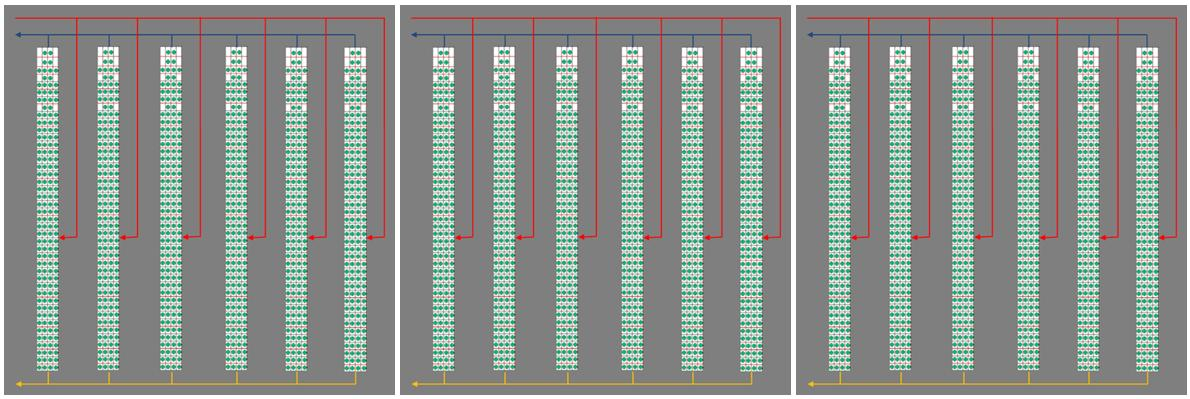
\includegraphics[height=0.1\textwidth]{cascade.png}
    \caption{Cascade}
    \label{fig:cascade}
    \end{figure}
How does one use thousands of fragile centrifuges in in a sensitive industrial process that doesn't tolerate even minor equipment hiccups? In order to achieve that, Iran uses a Cascade Protection System which is quite unique as it is designed to cope with ongoing centrifuge trouble by implementing a crude version of fault tolerance. The protection system is a critical system component for Iran’s nuclear program as without it, Iran would not be capable of sustained uranium enrichment.

The Cascade Protection System consists of two layers, the lower layer being at the centrifuge level.Three fast-acting shut-off valves are installed for every centrifuge at the connectors of centrifuge piping and enrichment stage piping. By closing the valves, centrifuges that run into trouble – indicated by vibration – can be isolated from the stage piping. Isolated centrifuges are then run down and can be replaced by maintenance engineers while the process keeps running. The central monitoring screen of the Cascade Protection System, which is discussed in detail in the last  section of this paper, shows the status of each centrifuge within a cascade – running or isolated – as either a green or a grey dot.
But the isolation valves can turn into as much of a problem as a solution. When operating basically unreliable centrifuges, one will see shut-offs frequently, and maintenance may not have a chance to replace damaged centrifuges before the next one in the same enrichment
stage gets isolated.
Iran found a creative solution for this problem, basically another workaround on top of the first workaround. For every enrichment stage, an exhaust valve is installed that allows for compensation of overpressure. By opening the valve, overpressure is relieved into the dump system. A dump system is present in any gas centrifuge cascade used for uranium enrichment but never used in production mode; it simply acts as a backup in case of cascade trips when the centrifuges must be evacuated and the “normal” procedure to simply use the tails take-off is unavailable for whatever reason. Iran discovered they can use (or abuse) the dump system to compensate stage overpressure. For every enrichment stage, pressure (controlling variable) is monitored by a pressure sensor. If that pressure exceeds a certain setpoint, the stage exhaust valve (controlled variable) is opened, and overpressure is released into the dump system until normal operating pressure is re-established – basic downstream control as known from other applications of vacuum technology.
    

\section{Description of the cyber-event}

    \begin{figure}[H]
    \centering
    \includegraphics[height=0.1\textwidth]{timeline.png}
    \caption{Timeline}
    \label{fig:timeline}
    \end{figure}

\section{Accident Analysis}
    \subsection{Event 1 - }
    \subsection{Event 2 - }
    
    
    \subsection{Event NA - }
    \subsection{Event NB - }
    
\section{Conclusion}


\begin{flushright}
Nicolò Diomedi
\end{flushright}
\\~\\
\begin{flushright}
Gabriele Gallotti
\end{flushright}
\\~\\
\begin{flushright}
Giacomo Minello\\

\includegraphics[scale=0.06]{figures/firmaMinello.png}
\end{flushright}

% print biblio with heading in the index
\newpage
\printbibliography[heading=bibintoc]
\end{document}
